% \begin{table}[!htbp]
\centering
\small 
\begin{tabular}{l|cccc}
\toprule
\textbf{Method} & \textbf{Multi} & \textbf{Open} & \textbf{Single} & \textbf{Temp}\\
\midrule
Flat Memory & 66.31 & 46.88 & 78.83 & 78.50 \\
Graph Memory & 66.67 & 48.96 & 80.50 & 76.64 \\  
\midrule
w/o Cross-Event & 66.31 & 46.88 & 80.86 & 79.44 \\
StructMem & 68.77 & 46.88 & 81.09 & 81.62 \\
\bottomrule
\end{tabular}
\caption{Paradigm comparison and ablation study on \texttt{LoCoMo} dataset.}
\label{tab:ablation}
\end{table}

\section{Experiments}
\subsection{Experimental Setup}
We first describe the dataset and evaluation metrics, followed by the baseline systems used for comparison. To ensure reproducibility, complete set of prompt templates and implementation details used for memory construction, question answering, and evaluation is provided in Appendix~\ref{appendix:prompts}.
\paragraph{Dataset and Metrics.} We evaluate on the \texttt{LoCoMo} benchmark~\cite{maharana2024evaluating} (see Appendix~\ref{dataset} for detailed statistics). Effectiveness is measured using LLM-as-a-judge evaluation; efficiency is measured by token usage, API calls, and runtime during memory construction.

\paragraph{Baselines.} We compare StructMem against RAG-based systems (OpenAI, FullContext, MiniRAG, LightRAG), flat memory methods (LangMem, A-Mem, Mem0), and structural memory methods (MemoryOS, Mem0$^\text{g}$, Zep, Memobase). All methods use gpt-4o-mini as the backbone and text-embedding-3-small for embeddings. Detailed retrieval and configuration parameters for all baselines are provided in Appendix~\ref{appendix:baseline}.

\subsection{Overall Performance}

Table~\ref{tab:locomo} shows StructMem achieves state-of-the-art overall performance on \texttt{LoCoMo}, with substantial gains in multi-domain and temporal reasoning where cross-event connections are critical for understanding causal relationships across dialogue sessions. Beyond effectiveness, StructMem demonstrates exceptional efficiency: compared to existing memory systems, it reduces token consumption and requires significantly fewer API calls, as our progressive structural organization avoids the expensive post-hoc graph construction. These results hold consistently across multiple judge models, as verified in Appendix~\ref{appendix:robustness}.

\subsection{Analysis}
We analyze StructMem from two complementary perspectives: a paradigm-level comparison that evaluates effectiveness and efficiency across all three memory paradigms, and an internal analysis that examines the mechanism underlying StructMem's reasoning gains.
\begin{figure*}[!t]
    \centering
    \subfigure[Token consumption over dialogue turns] { \label{fig:analysis_a} 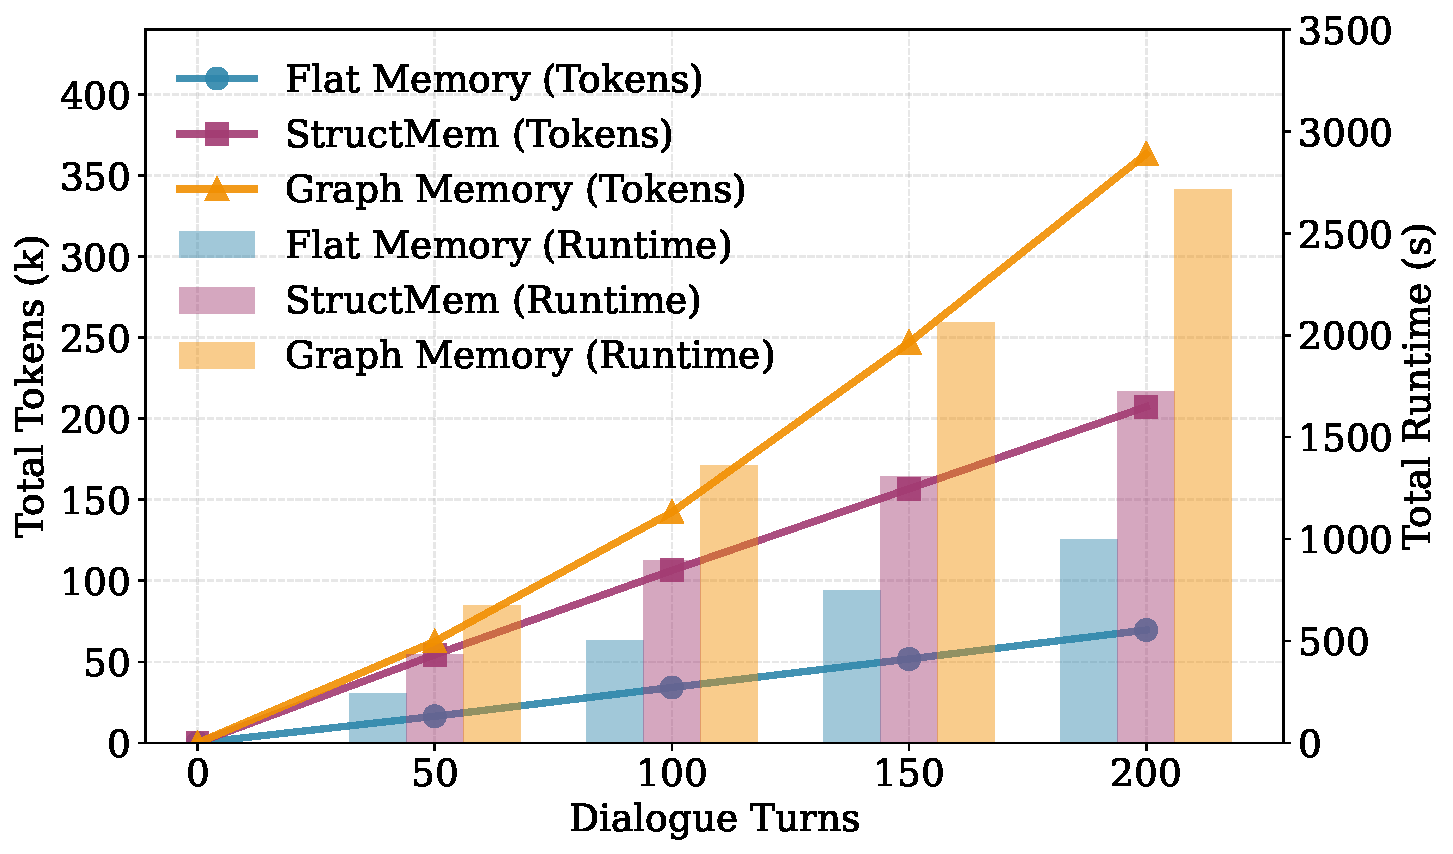
\includegraphics[width=0.49\linewidth]{figure/scalability_combined.pdf}}
    \subfigure[Component-wise token consumption] { \label{fig:analysis_b} 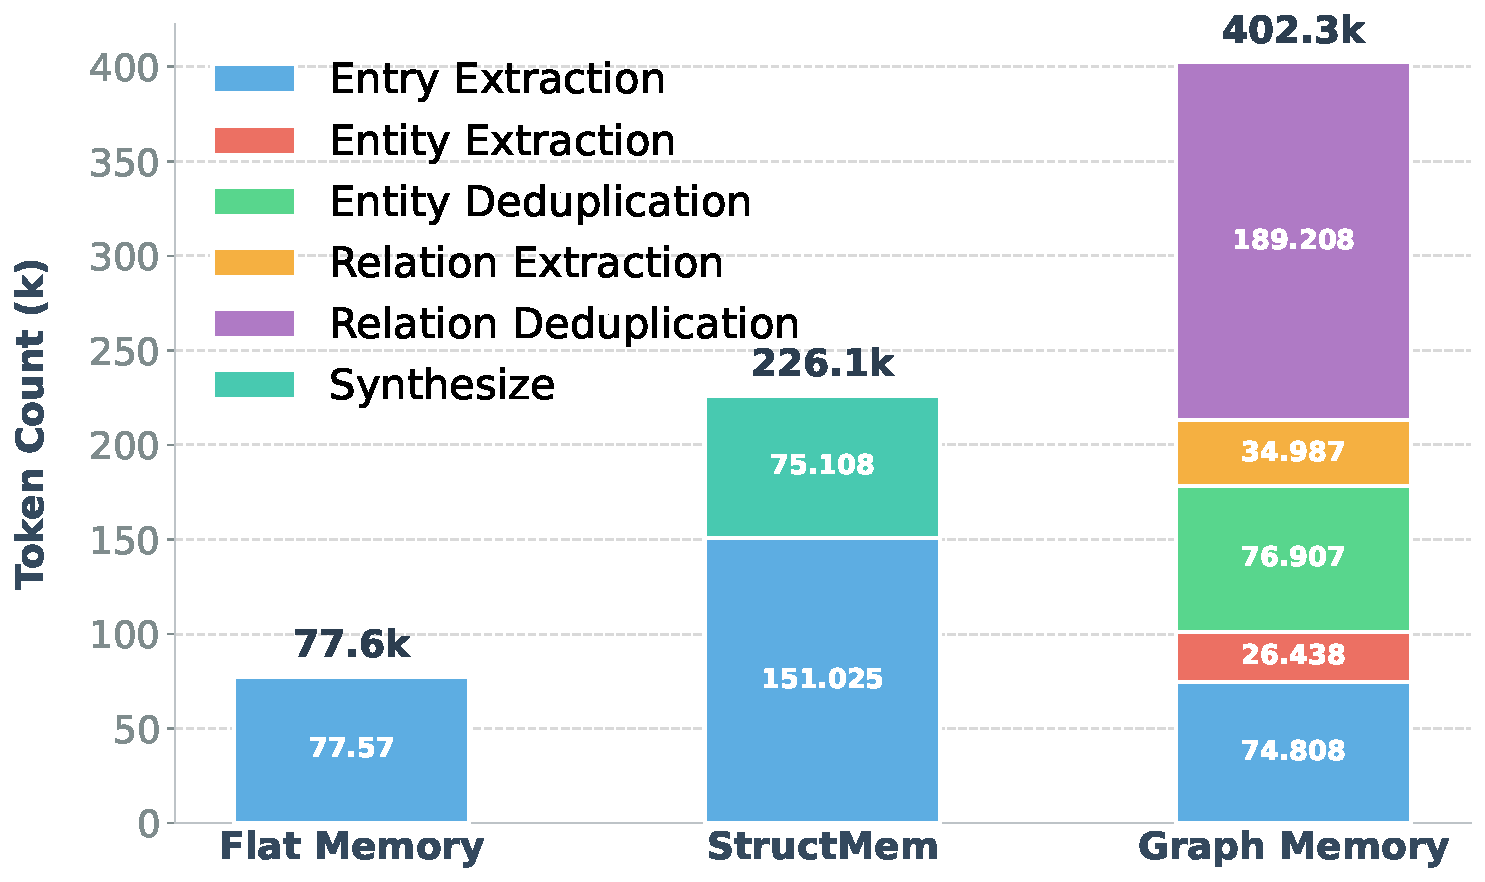
\includegraphics[width=0.49\linewidth]{figure/components_comparison.pdf}}
    \subfigure[Effect of the number of retrieved entries] { \label{fig:analysis_c} 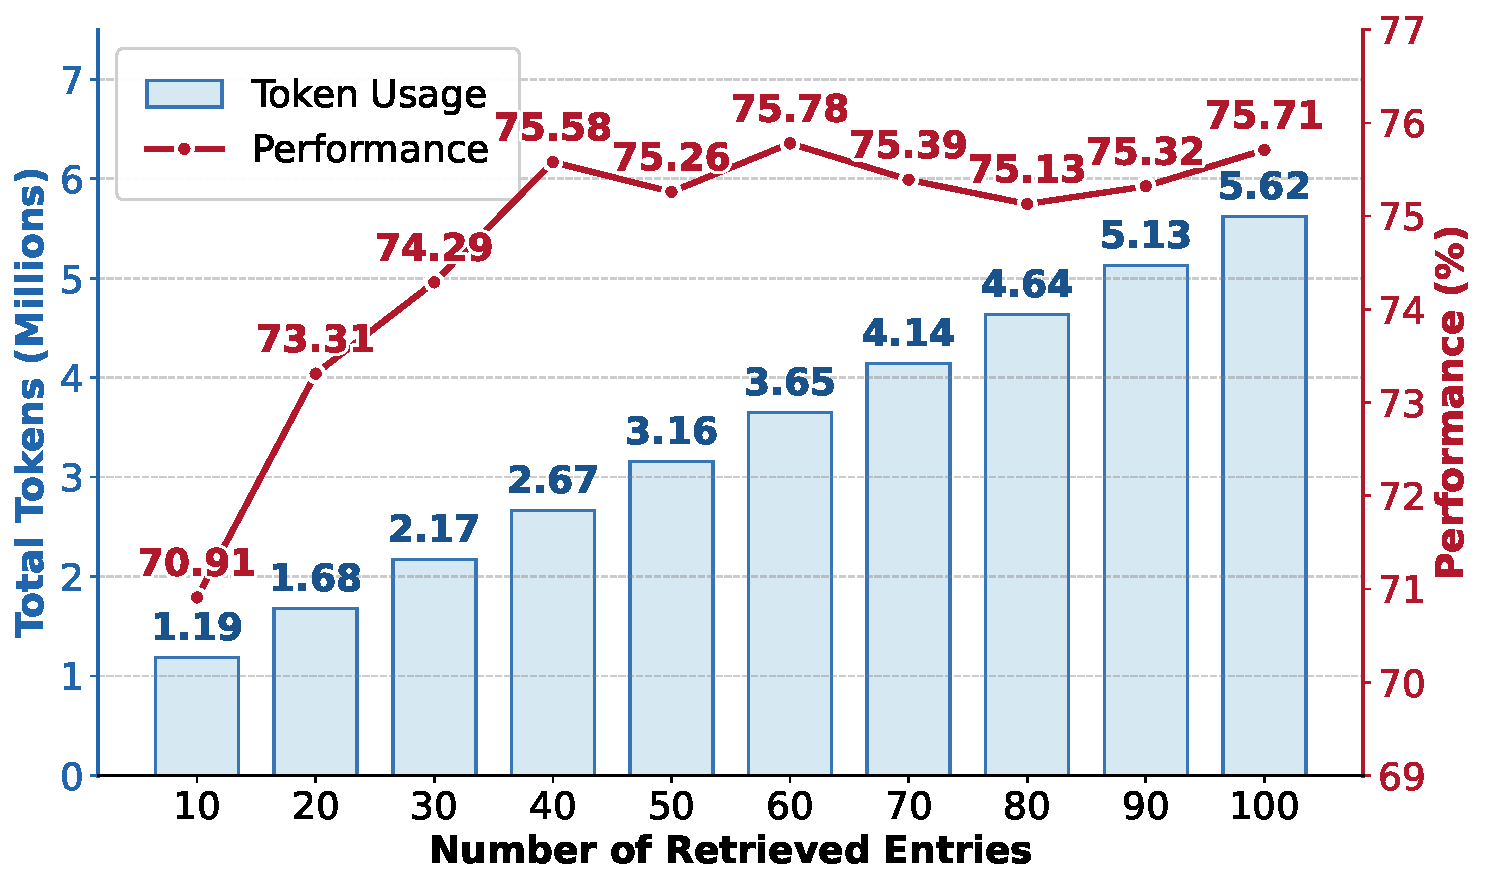
\includegraphics[width=0.49\linewidth]{figure/entry_retrieve_ablation_study.pdf}}    
    \subfigure[Effect of the number of semantic retrieval seeds $K$] { 
    \label{fig:analysis_d} 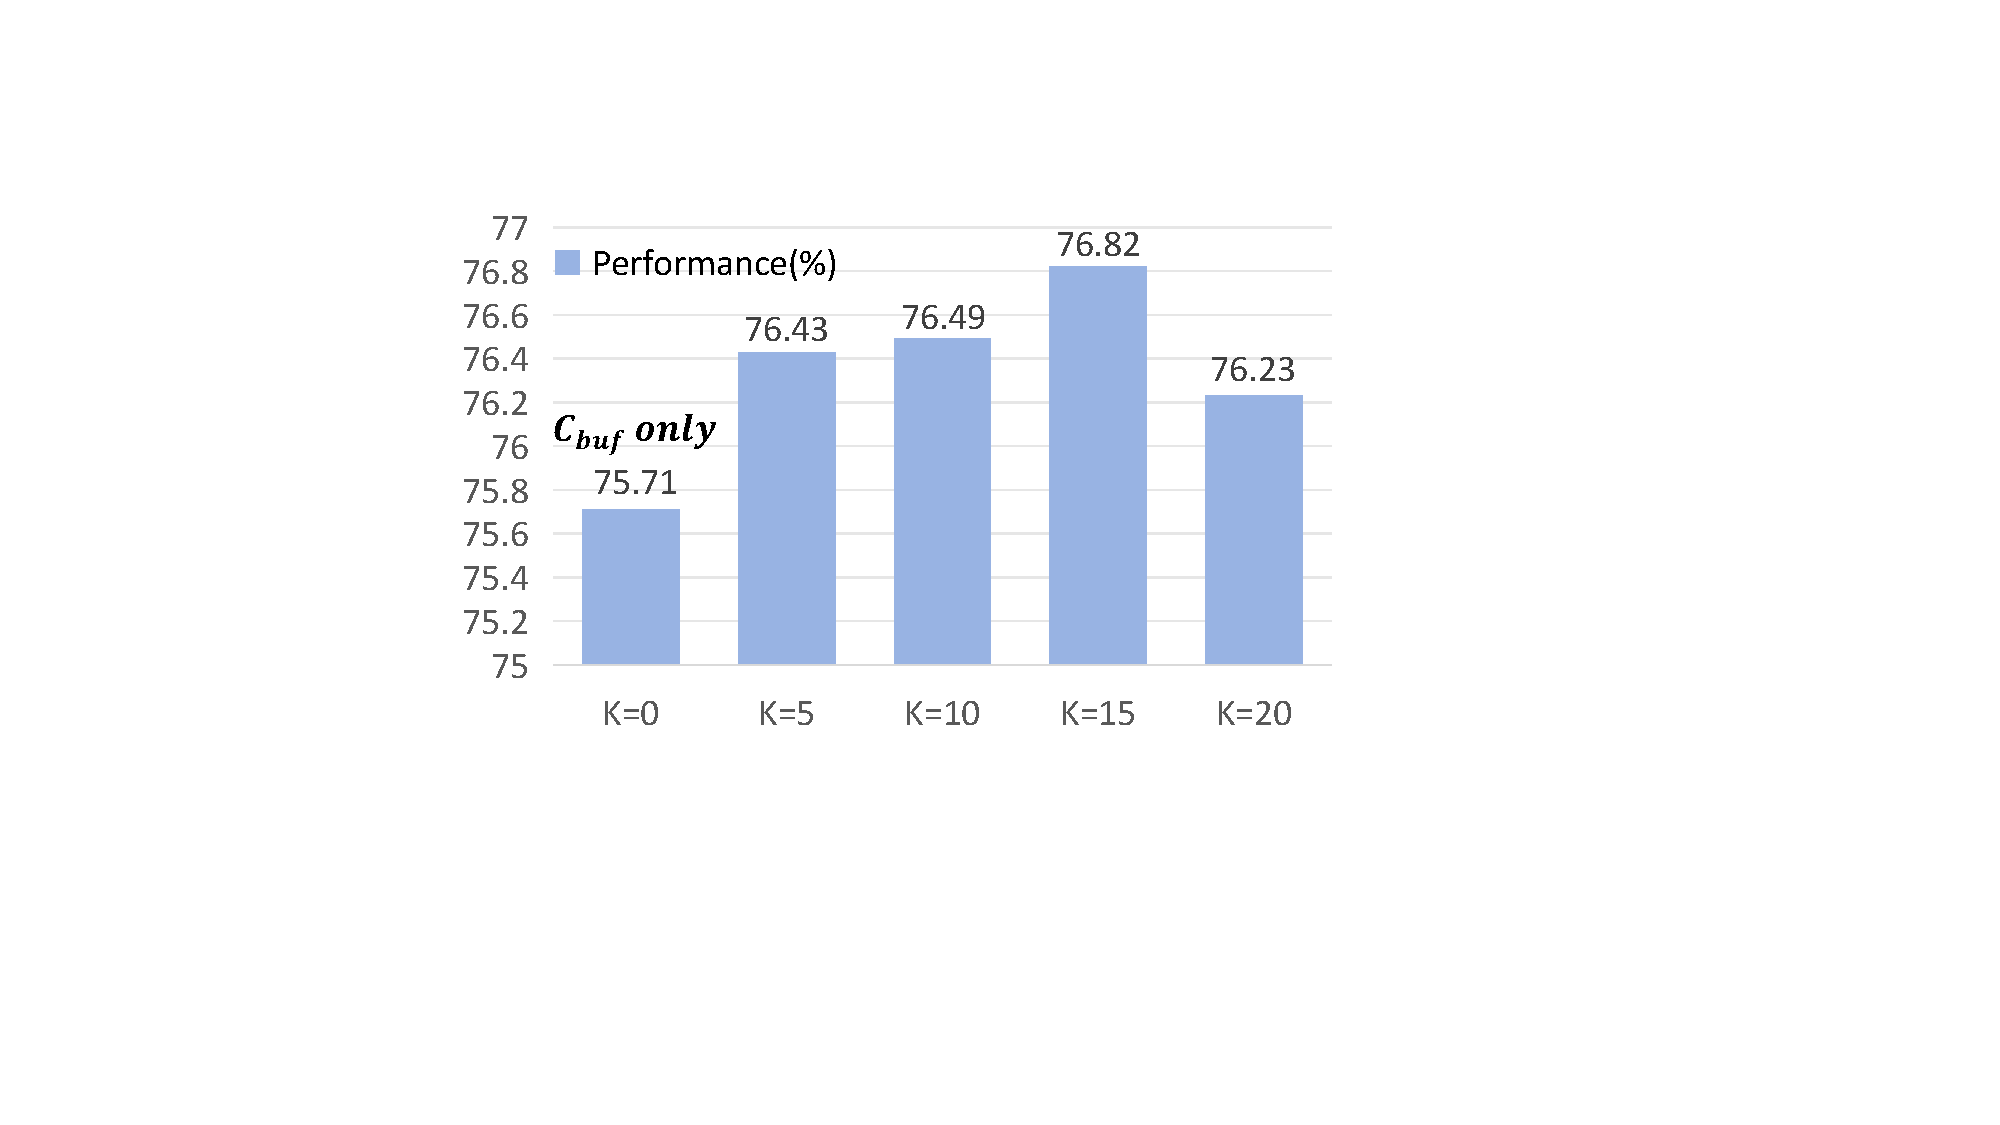
\includegraphics[width=0.49\linewidth]{figure/global_retrieve.pdf}}
    \caption{Analysis of efficiency across memory paradigms and internal mechanisms of StructMem.}
    \label{fig:analysis}
\end{figure*}
\paragraph{Paradigm Comparison.} 

\begin{table}[!htbp]
\centering
\small 
\begin{tabular}{l|cccc}
\toprule
\textbf{Method} & \textbf{Multi} & \textbf{Open} & \textbf{Single} & \textbf{Temp}\\
\midrule
Flat Memory & 66.31 & 46.88 & 78.83 & 78.50 \\
Graph Memory & 66.67 & 48.96 & 80.50 & 76.64 \\  
\midrule
w/o Cross-Event & 66.31 & 46.88 & 80.86 & 79.44 \\
StructMem & 68.77 & 46.88 & 81.09 & 81.62 \\
\bottomrule
\end{tabular}
\caption{Paradigm comparison and ablation study on \texttt{LoCoMo} dataset.}
\label{tab:ablation}
\end{table}

To validate the effectiveness of each paradigm, we conduct studies in Table~\ref{tab:ablation}. Starting from Flat Memory as the baseline, Graph Memory achieves improvements on single-session and open-domain tasks, though it decreases on temporal reasoning. In contrast, our approach demonstrates consistent improvements across all task types. Event-level structure improves performance in temporal reasoning and single-session. Cross-event structure yields further gains by capturing cross-temporal causal relationships.

To examine computational efficiency, we analyze token usage and runtime on the first conversation of \texttt{LoCoMo}. Figure~\ref{fig:analysis_a} shows that Graph Memory incurs significantly higher token usage and runtime as dialogue progresses. Figure~\ref{fig:analysis_b} reveals the source: graph construction requires four cascading LLM operations per event, with deduplication overhead growing quadratically. In contrast, StructMem achieves efficiency through buffered consolidation: by exploiting temporal locality, in which semantically related events naturally cluster within short time windows, the system accumulates events and processes them in batch during periodic synthesis. This effectively reduces cross-event organization from per-event operations to periodic batch processing, substantially cutting both API calls and token consumption.

\paragraph{StructMem Internal Mechanisms.} 
\label{Internal_Mechanisms}
We analyze whether hierarchical organization provides genuine reasoning gains beyond retrieval scaling. 

Figure~\ref{fig:analysis_c} reveals that flat retrieval performance peaks at 60 entries and plateaus thereafter, indicating that simply retrieving more atomic entries cannot improve effectiveness, as the bottleneck is knowledge reasoning rather than coverage. Cross-event consolidation addresses this by synthesizing semantically related events into higher-level relational hypotheses, creating information that does not exist in any individual memory entry.

Figure~\ref{fig:analysis_d} confirms this: without event connections ($K=0$), performance matches the flat retrieval plateau, but introducing cross-event synthesis yields substantial gains, demonstrating that hierarchical consolidation reconstructs causal relationships across temporal boundaries and enables fundamentally new reasoning capabilities. Fidelity analyses in Appendix~\ref{appendix:fidelity} further confirm that these synthesized connections are well-grounded, with minimal spurious associations.